\chapter{Modeling \& Simulation}
\section{Si:Ni-NPs formation }
\subsection{Homogenous nucleation\textsuperscript{[35][37]}}
In PS-PVD process, the Si and Ni powders are fed into plasma and evaporated immediately due to high temperature (>10,000K). Then, Si gas and Ni gas are co-condensed at the tail of plasma (2000$\sim$3000K). In particle formation, nucleation is the first and determining step. A Homogeneous nucleation occurs without any favorable nucleation site while heterogeneous nucleation occurs at a foreign surface. The necessary  physical quantities  and the corresponding symbol used in calculations in this chapter is demonstrated in and Table 3.1.
\begin{table}[h]
\caption{Physical quantity}
\centering
\begin{tabular}{ccc}
\toprule
Symbol & Physical quantity      & Dimension \\
\midrule
$I$    & Nucleation   frequency & $\mathrm{/m^{3}s}$    \\
$\alpha _{i}^{\ast }$ & Adsorption coefficient & -         \\
$S$  & Saturation ratio       & -         \\
$P_{\infty }$ & Saturation pressure    & Pa \\
 $k$ & Boltzmann constant     & J/K       \\
$T$  & temperature            & K         \\
 $\sigma $  & Surface energy   & $\mathrm{J/m^{2}}$\\
$m$ & Molecular mass         & kg        \\
$\rho $& Mass density           & $\mathrm{kg/m^{3}}$     \\
$n_{i}^{\ast }$ & critical density & /$\mathrm{m^{3}}$ \\
$r^{\ast }$ & critical radius & m \\
$L$ & Evaporation latent heat & J/mol \\
\bottomrule
\end{tabular}
\end{table}

\begin{table}[H]
\caption{Physical property\textsuperscript{[36]}}
\centering
\begin{tabular}{ccccccc}
\toprule
Atom & $T_{m}$(K) & $T_{b}$(K) & $\sigma$(mN/m)  & $\rho $($\mathrm{g/cm^{3}}$) & m(g/mol) & L(kJ/mol)\\
\midrule
Si   & 1680 & 3507 & 865  & 2.51 & 28.1 & 386 \\
Ni   & 1726 & 3110 & 1778 & 7.91 & 58.7 & 372\\
\bottomrule
\end{tabular}
\end{table}
There are two rival nucleation theories- the classical Becker-Doring theory and the revised Lothe-Pound theory. According to Becker-Doring theory, the nucleation frequency is  given by:
\begin{equation}
I=\frac{\alpha_{i}^{*} S P_{\infty}}{k T} \sqrt{\frac{2 \sigma}{\pi m}} \frac{m}{\rho} n_{i}^{*}  
\tag{3.1.1}
\end{equation}
The critical density $n_{i}^{\ast }$ is expressed as,
\begin{equation}
n_{i}^{*}=n_{1} \exp \left(-\frac{\Delta G^{*}}{k T}\right) 
\tag{3.1.2}
\end{equation}
where $n_{1}$ is the total number of atoms in the mother phase and $\Delta G^{*}$ is the energy barrier that an atom has to pass over in order to nucleation.
The occurrence of atomistic level events with the length scales on the order of $\sim$0.1 manometers and time scales of $10^{-13}$ seconds makes the nucleation a very complicated phenomenon to study. The  revised Lothe-Pound theory has taken the translational and rotational components of  the free energy of formation in to consideration.  By introducing a correction factor $\Xi_{i}^{*} $  , the critical density $n_{i}^{*}$ is given by following equation:
\begin{equation}
n_{i}^{*}=n_{1} \Xi_{i}^{*} \exp \left(-\frac{\Delta G^{*}}{k T}\right)  
\tag{3.1.3}
\end{equation}
With the expressions above, it has been possible to obtain an understanding of both homogeneous and heterogeneous nucleation. Based on our experiment, we focus the liquid-solid equilibrium system.
When a homogeneous nucleation takes place, there is a transformation from a small bubble of liquid to solid state, wherein two contributions to the change in the energy of the system: the energy decreases because the Gibbs energy of solid ($G_{S}$)  is lower than the energy of the liquid($G_{L}$) ; the energy increase is due to the birth of interface between the liquid and the vapor. The algebraic sum of such decrease and  increase is found to be the driving force for a nuclei formation. It shall be mentioned that the nucleation takes place at constant pressure and temperature.
The algebraic sum of  energy change during homogeneous nucleation is given by:
\begin{equation}
\Delta G=\frac{4 \pi r^{3}}{3} \Delta G_{V}+4 \pi r^{2} \sigma  
\tag{3.1.4}
\end{equation}
Where $r$ is the spherical nucleus of radius and $\sigma $ is the surface energy.
\begin{figure}[H]
\centering
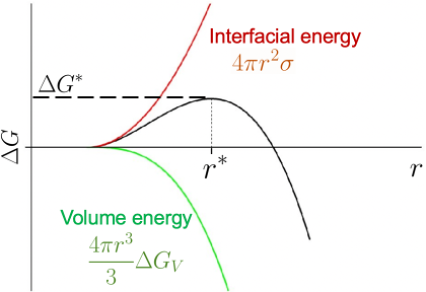
\includegraphics[width=8cm]{src/fig/fig31.png}
\caption{The energy change in nucleation\textsuperscript{[37]}}
\end{figure}
The total energy at first increases with increasing radius before reaching a maximum value at a critical radius $r^{*}$ and then decreasing (see Fig.3.1). The critical radius can be obtained by differentiating $\Delta G$ with respect to $r$, 
\begin{equation}
\frac{d \Delta G}{d r}=4 \pi r^{2} \Delta G_{V}+8 \pi r \sigma=4 \pi r\left(r \Delta G_{V}+2 \sigma\right)=0
\tag{3.1.5}
\end{equation}
By solving this,  $r^{*}$ is
\begin{equation}
r^{*}=-\frac{2 \sigma}{\Delta G_{V}}
\tag{3.1.6}
\end{equation}
Next,  we deal with the $\Delta G_{V}$ term.
The volumetric energy loss is:
\begin{equation}
\Delta G_{V}=G_{L}-G_{S}=H_{L}-H_{S}-T\left(S_{L}-S_{S}\right)
\tag{3.1.7}
\end{equation}
Where the $H$ is enthalpy and $S$ is entropy. Since phase transformation occurs at melting point $T_{m}$, that is, $\Delta G_{V}=0$. With denoting $H_{L}-H_{S}=\Delta H_{m}$, $S_{L}-S_{S}=\Delta S_{m}$, the term of $\Delta H_{m}$ equals  $T_{m}\Delta S_{m}$  at melting point.  Assume $\Delta H_{m}$ and $\Delta S_{m}$  are independent from temperature. Since nucleation needs driving force thus some overcooling is necessary.  
The derivation of above equations is,
\begin{equation}
\Delta G_{V}=\Delta H_{m}-T \Delta S_{m}=\Delta H_{m}-T \cdot \frac{\Delta H_{m}}{T_{m}}=\Delta H_{m} \frac{\Delta T}{T_{m}}
\tag{3.1.8}
\end{equation}
Substituting this expression into the eqn.(3.5) we get,
\begin{equation}
r^{*}=-\frac{2 \sigma T_{m}}{\Delta H_{m} \Delta T}
\tag{3.1.9}
\end{equation}
It’s clear that only a system with larger overcooling degree will be able to sustain a stable nucleation. 
Based information above, the energy barrier for a homogeneous nucleation is, 
\begin{equation}
\Delta G^{*}=\frac{16 \pi \sigma^{3}}{3 \Delta G_{V}^{2}}=\frac{16 \pi \sigma^{3} T_{m}^{2}}{3 \Delta H_{m}^{2} \Delta T^{2}}=\frac{4 \pi \sigma}{3}\left(r^{*}\right)^{2}
\tag{3.1.10}
\end{equation}
Here, the Kelvin equation is introduced to give the another expression of $r^{*}$ based on saturation mechanism.
\begin{equation}
r^{*}=\frac{2 \sigma v}{k T \ln S}
\tag{3.1.11}
\end{equation}
Here, $v$ is the volume of a droplet. Substituting this equation back with the assumption that $I =10^{22}$ ,  Then apply eqn.(3.1.2),(3.1.10),(3.11) into (3.1.1) ,  the following balance equation can be derived.
\begin{equation}
(\ln S)^{3}+\left(\frac{1}{2} \ln \left(\frac{\alpha_{i}^{*} P_{\infty}^{2} \Xi_{i}^{*}}{(k T)^{2} \rho I} \sqrt{\frac{2 \sigma m}{\pi}}\right)\right)(\ln S)^{2}-\frac{8 \pi \sigma^{3} v^{2}}{3(k T)^{3}}=0
\tag{3.1.12}
\end{equation}
We adopt the  $\Xi_{i}^{*}=10^{17}$ suggested by Lothe and Pound and assume adsorption coefficient  be 1, the $S$ can be calculated by applying all the physical properties shown in table 3.2. We denote this $S$ from calculation as theoretical value $S_{th}$.
On the other hand, $S$ can be expressed by its definition based on experimental condition. Assume at the time Si and Ni powders are fed into plasma they are evaporated immediately. Let partial pressure of each element, which can be calculated by feeding rate and chamber pressure, divide the corresponding theoretical saturated vapor pressure, we get the supersaturation $S_{n}$ experimentally\textsuperscript{[38]}.
Since both $S_{th}$ and $S_{n}$ are the functions of temperature, the intersection of two curves becomes the nucleation temperature. 
\begin{figure}[H]
\centering
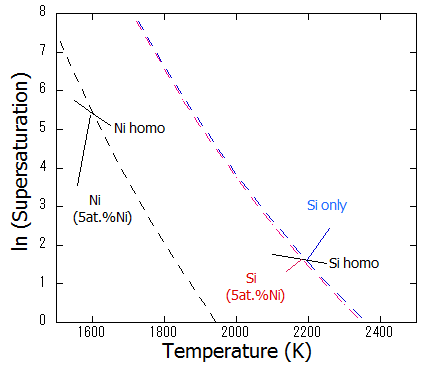
\includegraphics[width=8cm]{src/fig/fig32.png}
\caption{The homogeneous nucleation of Si and Ni in PS-PVD.}
\end{figure}

\begin{table}[H]
\caption{Homogeneous nucleation temperature of Si and Ni}
\centering
\begin{tabular}{ccc}
\toprule
Ni addition(at.\%) & $T_{N}^{Homo,Si}$(K) & $T_{N}^{Homo,Ni}$(K)     \\
\midrule
0                  & 2190 & -    \\
5                  & 2183 & 1604 \\
\bottomrule
\end{tabular}
\end{table}

\subsection{Heterogeneous nucleation\textsuperscript{[39]}}
The discussion so far has considered the homogeneous nucleation, which occurs spontaneously and randomly but requires supercooling.  In contrast,  heterogeneous nucleation occurs much more often in PS-PVD system because at some preferential sites, the effective surface energy is lower, thus diminishes the free energy barrier and facilitating nucleation. 
When heterogeneous nucleation occurs, to be specific, a cap-shaped liquid droplet  is deposited onto a solid surface, it will form a contact angle depending on its on surface tension as shown in fig.3.3
There are three different surface energies of interest:
\begin{itemize}
  \item $\sigma_{S L}^{A B}=(\text { solid } A-\text { liquid } B)$
  \item $\sigma_{L V}^{B}=(\text { vapor } \text { liquid } B)$
  \item $\sigma_{S V}^{A}=(\text { solid } A-\text { vapor })$
\end{itemize}
\begin{figure}[H]
\centering
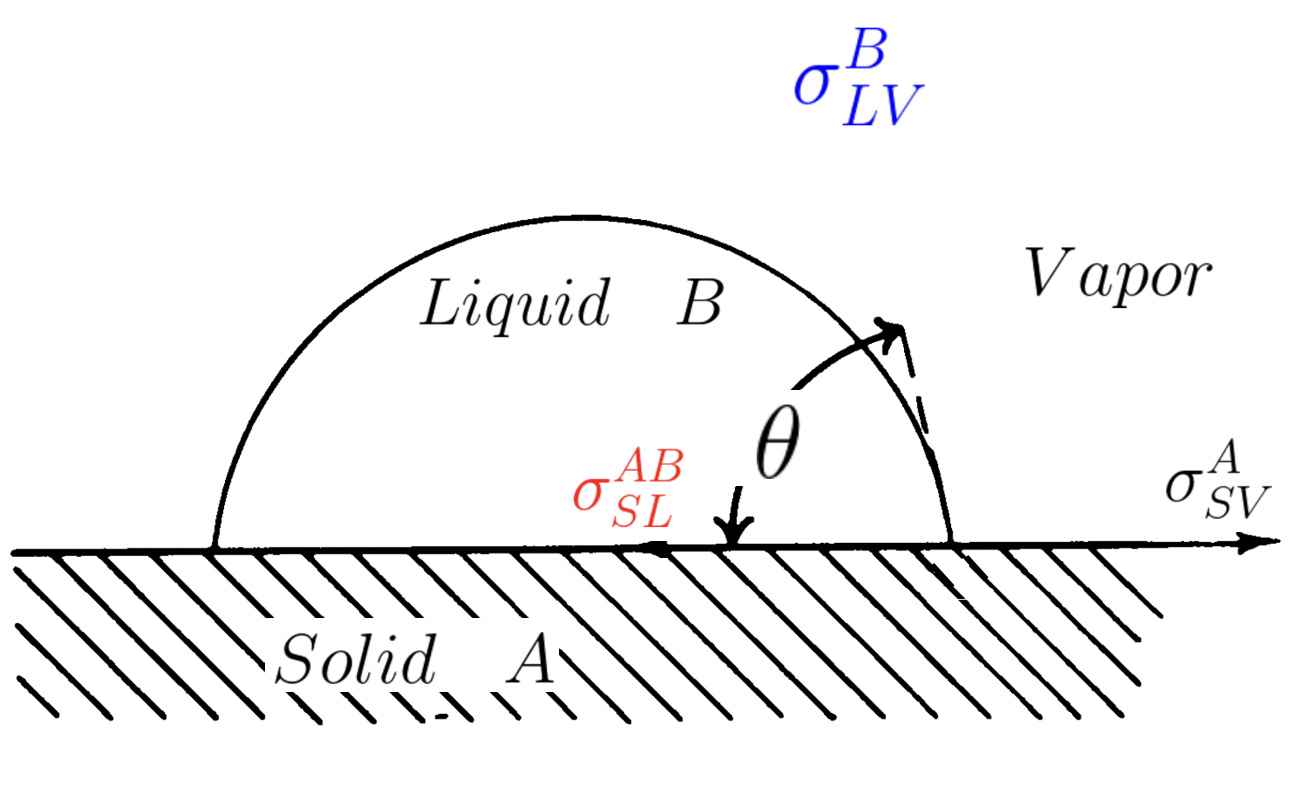
\includegraphics[width=8cm]{src/fig/fig33.5.png}
\caption{Surface tension}
\end{figure}
The contact angle $\theta $ can be  derived  in following equations:
\begin{equation}
\cos \theta=\frac{\sigma_{L V}^{A}}{\sigma_{L V}^{B}}-\frac{\lambda}{L_{e}^{B}}
\tag{3.1.13}
\end{equation}
Where  the $ \lambda $ represents solubility parameter and $L$ is the enthalpy of solution.
\begin{table}[H]
\caption{Enthalpy of solution\textsuperscript{[39]}}
\centering
\begin{tabular}{ccc}
\toprule
Solute & Solvent & Enthalpy of solution(kJ/mol) \\
\midrule
Si     & Ni      & -98                          \\
Ni     & Si      & -86                          \\
\bottomrule
\end{tabular}
\end{table}
According to Table 3.4,  we have  $ \lambda $ of -92 kJ/mol, which is the average of two enthalpies listed. 
Using the property values in Table 3.2 and Table 3.4, the contact angle of Ni droplet on a Si flat plane is,
\begin{equation}
\cos \theta=0.734
\tag{3.1.14}
\end{equation}
With the assumption that the surface energy of solid silicon is equal to liquid silicon. Next, consider the energy barrier for a heterogeneous nucleation. Here introduce the concept of shape factor,
\begin{equation}
f(\theta)=\frac{\cos ^{3} \theta-3 \cos \theta+2}{4}
\tag{3.1.15}
\end{equation}
With the same radius and same undercooling, the energy change by heterogeneous nucleation differs by such shape factor located outside the brackets of eqn.(3.4).
\begin{equation}
\Delta G=\left(\Delta G_{v} \frac{4}{3} \pi r^{3}+\sigma_{L V} 4 \pi r^{2}\right) \frac{\cos ^{3} \theta-3 \cos \theta+2}{4}
\tag{3.1.16}
\end{equation}
It is noteworthy that the critical radius $r^{*}$ remains unchanged for heterogeneous nucleation and homogeneous nucleation. Thus, the nucleation frequency $I$ can be expressed as,
\begin{equation}
I=\frac{\alpha_{i}^{*}\left(S P_{\infty}\right)^{2}}{(k T)^{2} \rho} \sqrt{\frac{2 \sigma m}{\pi}} \Xi_{i}^{*} \exp \left(-\frac{16 \pi \sigma^{3} v^{2}}{3(k T)^{3}(\ln S)^{2}} f(\theta)\right)
\tag{3.1.17}
\end{equation}
With the same assumption that $I =10^{22}$  and same substitution procedure in homogeneous case, the theoretical $S$ of  heterogeneous nucleation can be calculated .
However, this calculation is based on the simplification that Si particle surface is flat with respect to the heterogeneously formed nuclei. Practically, in the case of this PS-PVD experiment, Ni droplet is  expected to nucleate on solid Si nanoparticle in a spherical shape as fig.3.4 shows. 
\begin{figure}[H]
\centering
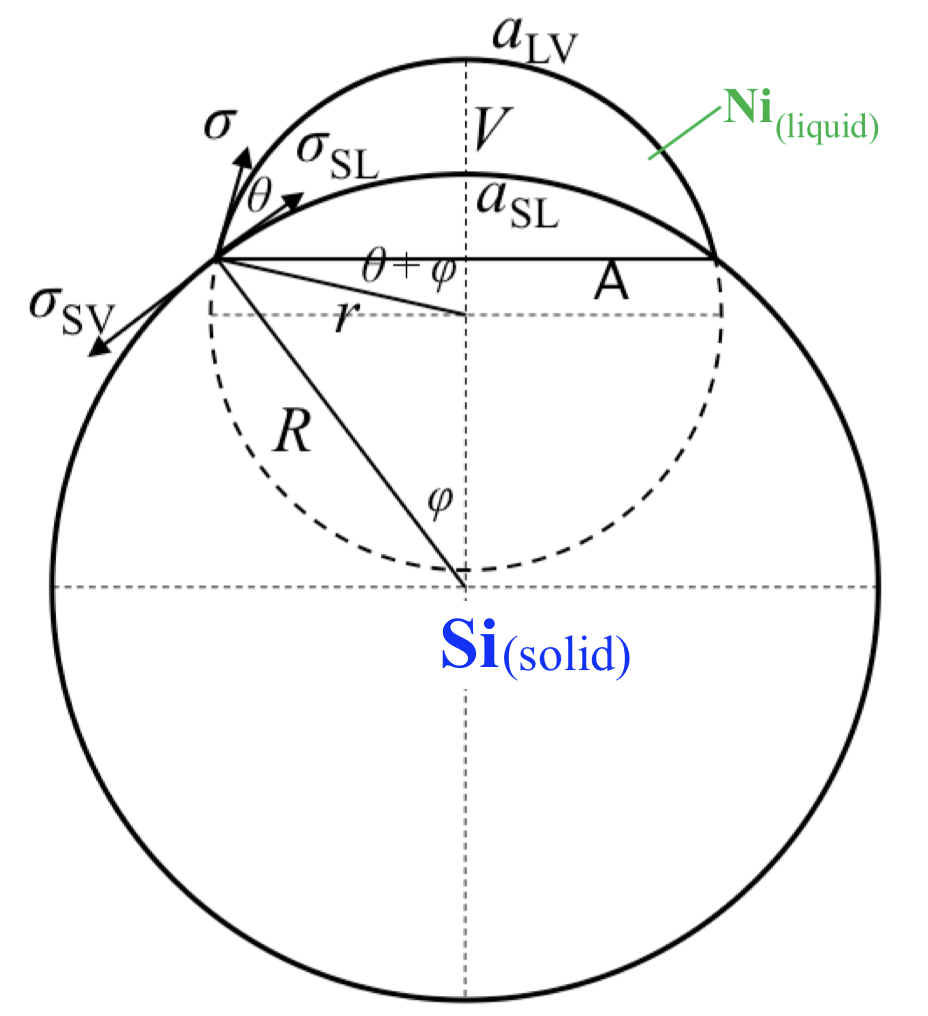
\includegraphics[width=8cm]{src/fig/fig33.png}
\caption{Schematic of heterogeneous nucleation on nanoparticles\textsuperscript{[40]}}
\end{figure}
As the diameter of Si nanoparticle changes, the shape factor changes accordingly. Fig.3.5 shows the shape factor $f(\theta)$ becomes a function of the diameter of Si nanoparticle, here $r^{*}$ =0.5 nm is assumed.
\begin{figure}[H]
\centering
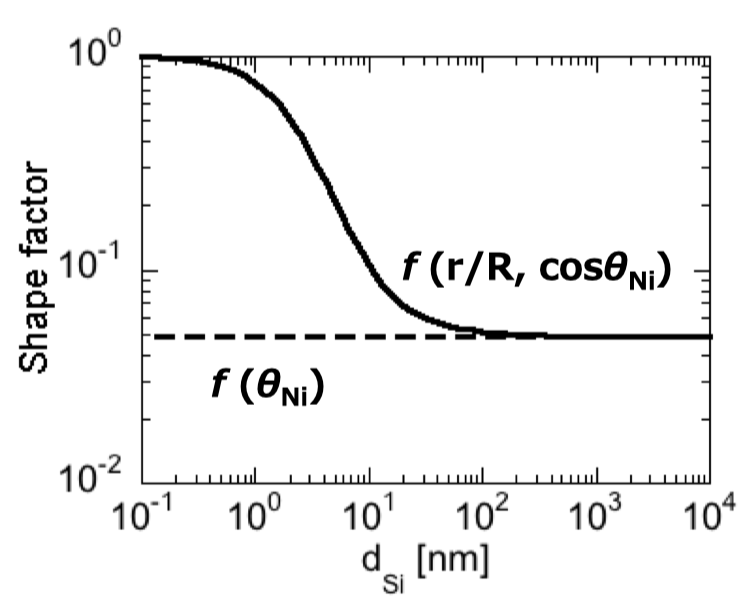
\includegraphics[width=8.5cm]{src/fig/fig34.png}
\caption{The shape factor of Ni on Si nanoparticle in different size}
\end{figure}
Fig.3.5 demonstrate that when $d_{Si}$ in the range of 0.1 $\sim$ 100 nm, shape factor undergoes a sharp drop, and when $d_{Si}$ > 100 nm, the shape factor becomes a constant, that is, $\cos \theta=0.734$, the same with the flat plane case. In addition, it's clear that  when heterogeneous nucleation takes place on smaller Si particles, the shape factor becomes large, and therefore the energy barrier becomes large, adding difficulties for Ni to nucleate on it. By applying different shape factor into calculation, the nucleation points of Ni on different-size Si particle is presented in Figure 3.6. As expected, the smaller Si particle is, the larger overcooling degree is needed for Ni to nucleate.

\begin{figure}[H]
\centering
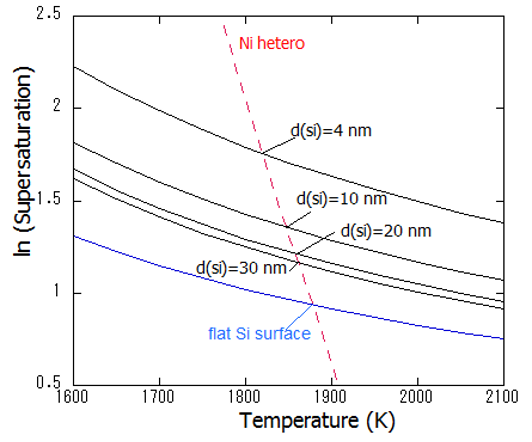
\includegraphics[width=8cm]{src/fig/fig35.png}
\caption{The size dependent heterogeneous nucleation of Ni on Si.}
\end{figure}
In each case the heterogeneous nucleation point of Ni on Si particle is in between $T_{N}^{Homo,Si}$(2183K) and $T_{N}^{Homo,Ni}$(1604K), 
holding the sequence of 
$$\boxed{T_{N}^{Homo,Si}>T_{N}^{Hetero,Ni}>T_{N}^{Homo,Ni}}$$
Only in this sequence can we obtain the target Si:Ni nanostructure.

\subsection{Particle growth\textsuperscript{[36]}}
There are two types of particle growth after nucleation: (1) The coagulation by adsorption of vapour atoms/molecules on the particle surface. (2) The coagulation by collision-coalescence of particles. However, the former is credible only in really initial stages of particle growth, i.e. when their diameters are of order 1 nm. In the case of our PS-PVD processing particle,  such approximations are obviously not possible. Therefore, the latter called collision-coalescence theory is used.

In collision-coalescence theory, there are two approaches: (1) the Collision Rates Continuum Theory, which is treated as a diffusion problem, and (2) the Free Molecule Theory based on the noble gas particle kinetics.  When the ratio of mean free path to particle radius is <0.1, the former is used.  If such ration >10, the latter is used. In our case, the mean free path is $\sim$850 nm, as will be described later, so the Free Molecule Theory can be applied for particle size up to 140 nm. From the experimental results, the primary particle size  satisfy this size requirement, the  Free Molecule Theory  is used.

In a system of  three classes of gases colliding with each other, the mean free path of  particular gas 1  can be expressed as,

\begin{equation}
\begin{split}
\lambda_{1 \rightarrow 1,2,3} &= \frac{\bar{c}_{1}}{\Gamma_{1 \rightarrow 1,23}}\\
&=\frac{1}{\pi\left(\sqrt{2} \sigma_{1}^{2} N_{1}+\left(\frac{\sigma_{1}+\sigma_{2}}{2}\right)^{2} N_{2} \sqrt{1+\frac{m_{1}}{m_{2}}}+\left(\frac{\sigma_{1}+\sigma_{3}}{2}\right)^{2} N_{3} \sqrt{1+\frac{m_{1}}{m_{3}}}\right)}\\
\end{split}
\tag{3.1.18}
\end{equation}
Where $c$ represents the speed, $\sigma $ represents the collision diameter, $\Gamma $represents the collision frequency.
Apply the collision diameter listed in table3.? to equation the mean free path  of Si can be  obtained. $\lambda_{Si}=\sim 850$ nm. To satisfy the Free molecule theory the Si particle should be smaller than 170 nm. In addition, it’s difficult for Ar or H atom to be included into a Si particle, so we can just focus on the case of Si collide with each other. Then $\lambda_{Si}$ can be reduced to $\sim 400 \mu m$. This enlarge the requiring Si particles size to several micro meters. 

\begin{table}[H]
\caption{collision diameter\textsuperscript{[37]}}
\centering
\begin{tabular}{cc}
\toprule
Molecule &  $\sigma$(\AA) \\
\midrule
Si       & 3.046 \\
Ar       & 3.432 \\
H        & 2.915 \\
\bottomrule
\end{tabular}
\end{table}
Next, consider the collision between larger particles. 
The collision frequency of particles consisting of i atoms and particles consisting of j atoms is,
\begin{equation}
L_{i j}=\left(8 \pi k T \frac{m_{i}+m_{j}}{m_{i} m_{j}}\right)^{\frac{1}{2}}\left(R_{i}+R_{j}\right)^{2} N_{i} N_{j}
\tag{3.1.19}
\end{equation}
Where $m$ is the mass, $R$ is the radius and $N$ is the particle number concentration.
Differentiating $N$ with respect to $t$(time) gives,
\begin{equation}
\frac{d N}{d t}=\sum_{i=1}^{\infty} \frac{d N_{i}}{d t}=c\left(\sum_{i=1}^{\infty} \sum_{j=1}^{i-1} \frac{1}{2} L_{j(i-1)}+\frac{1}{2} \sum_{i=1}^{\infty} L_{ii}-\sum_{i=1}^{\infty} \sum_{j=1}^{\infty} L_{i j}\right)
\tag{3.1.20}
\end{equation}
$c$ represents the sticking coefficient.
Assume the particles are the same size,to say, $i = j$.  eqn. (3.20) can be rewritten as:
\begin{equation}
\frac{d N}{d t}=-\frac{c}{2}\left(\frac{16 \pi k T}{m}\right)^{\frac{1}{2}}(2 R)^{2} N^{2}
\tag{3.1.21}
\end{equation}
Note that the following relationships  constantly hold:
\begin{equation}
m=\frac{4}{3} \pi R^{3} \rho
\tag{i}
\end{equation}
\begin{equation}
N=\frac{3 C_{0} M}{4 \pi R^{3} \rho N_{A}}
\tag{ii}
\end{equation}
$C_{0}$  is the concentration of molecules and $m$ is the molecular weight.
Substitute the $m$ and $N$ above into eqn. (3.21) we have,
\begin{equation}
\frac{d N}{d t}=-4 c\left(\frac{3 k T}{\rho}\right)^{\frac{1}{2}}\left(\frac{3 M}{4 \pi \rho N_{A}}\right)^{\frac{1}{6}} C_{0}^{\frac{1}{6}} N^{\frac{11}{6}}
\tag{3.1.22}
\end{equation}
In PS-PVD, the temperature will decrease with time. So we introduce the cooling rate $\varepsilon $ (K/s),
\begin{equation}
T=T_{0}-\varepsilon t
\tag{3.1.23}
\end{equation}
Applying this temperature profile into eqn. (3.22) and by solving this differential equation, the particle number concentration can be obtained.
\begin{equation}
N=N_{0}\left(1+\frac{20 \sqrt{3}}{9} c\left(\frac{k}{\rho}\right)^{\frac{1}{2}}\left(\frac{3 M C_{0}}{4 \pi \rho N_{A}}\right)^{\frac{1}{6}} \frac{1}{\varepsilon}\left(T_{0}^{\frac{3}{2}}-\left(T_{0}-\varepsilon t\right)^{\frac{3}{2}}\right) N_{0}^{\frac{5}{6}}\right)^{-\frac{6}{5}}
\tag{3.1.24}
\end{equation}
However, $\varepsilon $ is a function of time instead a constant. For convenience, an analytical solution is obtained with incorporation of $\varepsilon (t)$ and the assumption of sticking coefficient $c=1$.
The analytical solution  is carried out with setting proper step size of the variable,namely, $t$. In each step size the cooling rate is constant. Let $T_{0}$ and  $T_{1}$ be the initial and final temperature, respectively. And we have the cooling rate as,
\begin{equation}
\varepsilon=\frac{T_{0}-T_{1}}{\Delta t}
\tag{3.1.25}
\end{equation}
By replacing the initial value of $N$ repeatedly, analytical solution of $N$ is obtained. 
Using this particle number concentration, we can calculate the particle size with the relationship between the existing Si atoms, the density of Si atoms in a particle and the volume of a Si atom.
\begin{figure}[H]
\centering
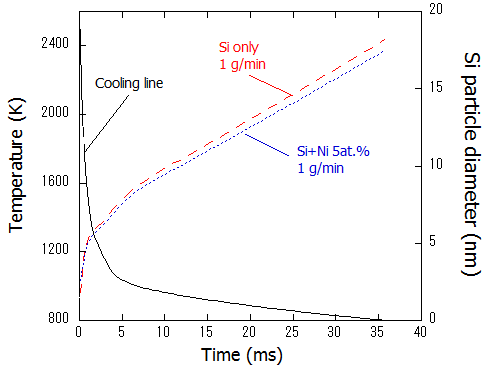
\includegraphics[width=9cm]{src/fig/fig36..png}
\caption{Si particle growth}
\end{figure}
As Fig.3.7 shows, the final diameter of Si primary particle in PS-PVD is 20nm.

\newpage
\section{CNT growth in PE-CVD}
\subsection{Mathematical model of CNT growth\textsuperscript{[41]}}
\begin{table}[H]
\centering
\caption{Physical quantity for CNT growth simulation}
\begin{tabular}{@{}lcc@{}}
\toprule
Description                                                                  & symbol   & unit      \\ \midrule
Initial concentration of feedstock gas                                       & $n_{0}$  & $m^{-3}$  \\
Volumetric number density of  $\mathrm{C_{2}H_{2}}$                             & $n$      & $m^{-3}$  \\
Volumetric number density of pyrolysis product $\mathrm{C_{4}H_{4}}$            & $n_{p}$  & $m^{-3}$  \\
Mass of $\mathrm{C_{2}H_{2}}$                                                & $m$      & kg        \\
Mass of $\mathrm{C_{4}H_{4}}$                                                & $M$      & kg        \\
Surface area of catalyst(Ni) particle                                        & $S_{0}$  & $m^{2}$   \\
Particle flux of  $\mathrm{C_{2}H_{2}}$ to Ni surface                         & $F_{b1}$ & $s^{-1}$  \\
Particle flux of $\mathrm{C_{4}H_{4}}$ to Ni surface                          & $F_{b2}$ & $s^{-1}$  \\
Particle flux of Carbon provided by $\mathrm{C_{2}H_{2}}$                    & $F_{c1}$ & $s^{-1}$  \\
Particle flux of Carbon provided by $\mathrm{C_{4}H_{4}}$                    & $F_{c2}$ & $s^{-1}$  \\
Coefficients relating to $\mathrm{C_{2}H_{2}}$ sticking and geometric process  & $p_{1}$  & -         \\
Coefficients relating to $\mathrm{C_{2}H_{2}}$ sticking and geometric process & $p_{1}$  & -         \\
Carbon atoms on the surface                                                  & $N_{C}$  & -         \\
Carbon atoms converted to carbonaceous layer                                 & $N_{L1}$ & -         \\
Inactive Ni atoms                                                            & $N_{L2}$ & -         \\
Carbon atoms diffused into bulk Ni                                           & $N_{B}$  & -         \\
Carbon atoms incorporated into CNT                                           & $N_{T}$  & -         \\
Rate constant of surface–bulk penetration of Carbon                          & $k_{sb}$ & $s^{-1}$  \\
Rate constant of bulk diffusion of Carbon in Ni                              & $k_{b}$  & $s^{-1}$  \\
Rate constant of aurface diffusion of Carbon on Ni                           & $k_{s}$  & $s^{-1}$  \\
Rate constant of precipitation of carbon into  CNT                           & $k_{t}$  & $s^{-1}$  \\
Rate constant of carbonaceous layer formation                                & $k_{c1}$ & $s^{-1}$  \\
Rate constant of carbonaceous layer dissolution                              & $k_{d1}$ & $s^{-1}$  \\
Number of monolayers in MWCNT                                                & $\alpha$ & -         \\
Number density of Carbon atoms on a monolayer                                & $n_{m}$  & $cm^{-2}$ \\
Number density of Carbon atoms per length                                    & $z$      & $cm^{-1}$ \\ \bottomrule
\end{tabular}
\end{table}
The earliest growth mechanisms of CNTs is established by Baker\textsuperscript{[18]}. In recent decades, several research groups have published many models with a better understanding of the growth mechanisms. They are all more or less based on the same processes, including adsorption and dissolution of carbon species at the metal catalyst particle, surface or bulk diffusion nanostructure nucleation and growth. Most of these models are applied to CNT growth by thermal CVD, but some are applied also for PE-CVD, and in general the principles are the same for both growth techniques.

In the case of Si:Ni-NPs as the substrate to grow CNT, where the Ni is directly attached to Si nanoparticle and it is expected to be the catalyst. However, even plasma is utilized to provide a low-temperature growth condition, this Si:Ni template is different from those in literature, for there is no diffusion barrier in between Si and Ni. That is, Ni silicidation is inevitable at elevated temperature. Therefore,  the Ni atoms will diffuse into Si while CNT grow on Ni, which may early terminate CNT without attain to the expected length.  
For convenience, we first concentrate on the move of carbon atoms, assuming Ni silicidation is not occurred at elevated temperature. Through this way can we establish a fundamental modelling of CNT and thereby revise it with adding the Ni-silicidation effect. 
The CNT growth model is  based on the thermal CVD\textsuperscript{[41]} applying to all temperature range.  By focusing the balance of carbon particles at different location, the length of carbon nanotubes becomes a function of annealing time. There are two competitive processes that contribute to the CNT growth and termination. For positive growth, the feed stock gas $\mathrm{C_{2}H_{2}}$ decompose into carbon atoms that diffuse in catalyst bulk and on surface then incorporate into carbon nanotubes. For negative termination, the excessive decomposed carbon atoms from $\mathrm{C_{2}H_{2}}$ form a carbonaceous layer that reduce the active catalyst surface. Also, a small fraction of $\mathrm{C_{2}H_{2}}$ convert into its pyrolysis product, which contains excessive carbon atoms per molecule. Such pyrolysis product contributes to pyrolysis product. If the temperature is high enough, some extra reactions take place, for instance, catalyst poisoning, that contribute to termination as well. 
\begin{figure}[H]
\centering
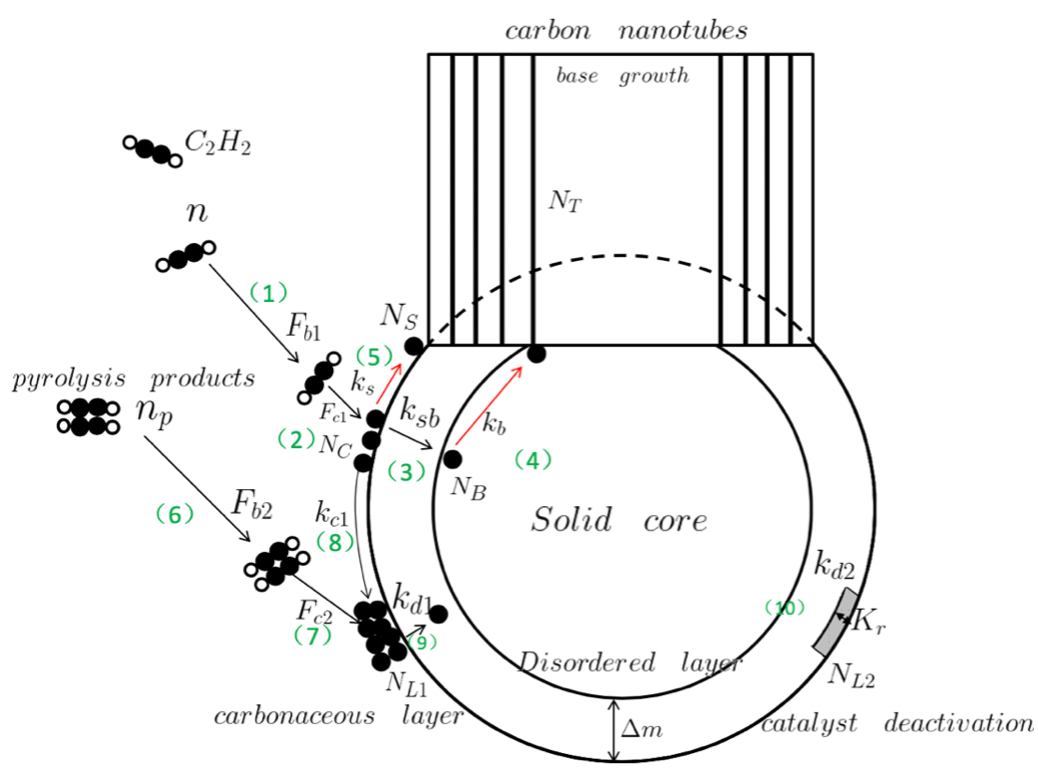
\includegraphics[width=12cm]{src/fig/fig37.png}
\caption{Schematic representation of processes responsible for feeding and termination of CNT growth. The number in bracket represents specific reaction\textsuperscript{[41]}.}
\end{figure}
As Fig.3.8 shows, the moving of carbon-containing species are divided into elementary processes and each are described by a single rate constant in an Arrhenius form.
The catalyst particle is regarded as a sphere, of which the initial surface area is:
\begin{equation}
S_{0}=4 \pi r^{2}
\end{equation}
With the carbonaceous layer forming, the exposed surface is reduced and expressed in terms of effective surface. 
\begin{equation}
S=\left(1-\frac{N_{L}}{\alpha S_{0} n_{m}}\right)S_{0}
\end{equation}
$\alpha $ is the number of monolayers, $n_{m}={10}^{15} m^{-2}$ is the surface density of a monolayer of carbon atoms.
\\
(1) The $\mathrm{C_{2}H_{2}}$  flux physically impinge to catalyst surface $F_{c1}$ following Hertz–Knudsen equation. 
\begin{equation}
F_{b 1}=\frac{1}{4} S_{0} n\left(\frac{k_{\mathrm{B}} T}{2 \pi m}\right)^{1 / 2}
\tag{3.2.1}
\end{equation}
(2) Only a fraction of impinging $\mathrm{C_{2}H_{2}}$ flux can be chemically absorbed and decomposed by catalyst. Assume the coefficients relating to $\mathrm{C_{2}H_{2}}$ sticking and geometric process $p_{1}=1$.  The decomposition reaction, of which the rate constant is $k_{de1}$ and decomposition energy barrier $E_{de1}$ , provides primary carbon atoms $N_{C}$ on the surface of catalyst.
\begin{equation}
F_{c 1}=p_{1}F_{b1}\exp \left(-E_{d e 1} / k_{B} T\right)
\tag{3.2.2}
\end{equation}
Assuming this decomposition is $0^{th}$ order reaction(gas concentration independent), So the decomposition rate constant $k_{de1}$ can be derived as,
\begin{equation}
k_{d e 1}=\frac{S_{0}}{p_{1}} \frac{1}{4} n \sqrt{\frac{k_{B} T}{2 \pi m}} \exp \left(-E_{d e 1} / k_{B} T\right)
\tag{3.2.3}
\end{equation}
(3) Surface-bulk penetration of carbon atoms with the rate constant, $k_{sb}$:
\begin{equation}
k_{s b}=B \exp \left(-E_{s b} / k_{B} T\right)
\tag{3.2.4}
\end{equation}
(4) Bulk diffusion of carbon atoms: the rate determining step in typical thermal CVD. assume that dissolution of carbon atoms will form a highly disordered ‘molten’ layer on the surface with thickness $\delta m$, expressed in the number of carbon monolayers denes the number of CNT walls. Note that the term ’bulk’ refers to the molten layer, because with the assumption of molten layer in between surface and sold core, carbon atoms will not diffuse further into solid core to prevent unnecessary paths. After diffusing and migrating to nucleation site, the carbon atoms $N_{B}$, is absorbed immediately into $N_{T}$ with a kinetic rate constant $k_{b}$. To quantify $k_{b}$ , consider the characteristic time for bulk diffusion[ref6].
\begin{equation}
\tau_{b} \approx l^{2} / D_{b}
\tag{3.2.5}
\end{equation}
where $l$ is the characteristic path length of diffusing species. For a spherical medium $l=r$,  $D_{b}$ is the bulk diffusion coefficient. Thus, the bulk diffusion rate constant $k_{b}$ can be expressed as:
\begin{equation}
k_{b}=\frac{D_{b 0}}{r^{2}} \exp \left(-E_{b} / k_{B} T\right)
\tag{3.2.6}
\end{equation}
(5) Surface diffusion of carbon atoms on catalyst surface, nucleation, and carbon atoms continuous incorporation into $N_{T}$. Generally, before growth can start, nucleation has to take place. If the growth process is the rate controlling step, a continuous acceleration should be observed in the early stages of the deposition. 
\begin{equation}
k_{s}=\frac{D_{s 0}}{r^{2}} \exp \left(-E_{s} / k_{B} T\right)
\tag{3.2.7}
\end{equation}
It’s noteworthy that bulk diffusion(step(3)-(4)) and surface diffusion (5) are parallel routes.  It has been often stated in the literature  that the surface diffusion may be the main processes enabling a rapid, low-temperature growth of CNTs, or more preciesly, CNFs, due to the low temperature. On the contrast,at relatively high substrate temperatures (T>500\(^\circ\)C), the dominant carbon diffusion will be the bulk diffusion. The details is discussed in next section. 

After completing nucleation, a continuous decline in rate would be expected, as the area available for the gas reaction is progressively reduced by the growth of carbon on it. The termination of CNT is determined by excessive carbon atoms that form carbonaceous layer that contains $N_{L1}$ carbon atoms. In addition, at higher temperature  (>700\(^\circ\)C), some mechanisms that are responsible for the catalytic deactivation should be taken into account. For instance, poisoning, due to gas-phase pyrolysis products; formation of metal carbide; catalyst oxidation, etc.
\\

\noindent (6) The carbonaceous layer containing $N_{L1}$ carbon atoms is partly formed by impingement, chemisorption, catalytic decomposition of pyrolysis products. The pyrolysis product can be $\mathrm{C_{4}H_{4}}$, $\mathrm{C_{6}H_{6}}$, etc. For simplification, we consider $\mathrm{C_{4}H_{4}}$ only. This process is the same with step (1), only the subject is different. The impinging  $\mathrm{C_{4}H_{4}}$ flux onto the catalyst surface is,
\begin{equation}
F_{b 2}=\frac{1}{4} S_{0} n_{p}\left(\frac{k_{\mathrm{B}} T}{2 \pi M}\right)^{1 / 2}
\tag{3.2.8}
\end{equation}
(7) The pyrolysis product $\mathrm{C_{4}H_{4}}$ undergoes samely  chemisorption, catalytic decomposition in step(2). Assume coefficient $p_{2}=1$ and denote decomposition energy barrier of pyrolysis product as $E_{de2}$.
\begin{equation}
F_{c 2}=p_{2}F_{b2}\exp \left(-E_{d e 2} / k_{B} T\right)
\tag{3.2.9}
\end{equation}
So the related decomposition rate constant $k_{de2}$ can be derived as,
\begin{equation}
k_{d e 2}=\frac{S_{0}}{p_{2}} \frac{1}{4} n_{p} \sqrt{\frac{k_{B} T}{2 \pi M}} \exp \left(-E_{d e 2} / k_{B} T\right)
\tag{3.2.10}
\end{equation}
(8) Part of $N_{C}$ carbon atoms are integrated into  carbonaceous layer.
\begin{equation}
k_{c l}=G \exp \left(-E_{c l} / k_{B} T\right)
\tag{3.2.11}
\end{equation}
(9) This carbonaceous layer could be partially dissolved by the catalyst.
\begin{equation}
k_{d s 1}=H \exp \left(-E_{d s 1} / k_{B} T\right)
\tag{3.2.12}
\end{equation}
(10) As for the extra reactions at higher temperature, assign a rate constant,$K_{r}$, to undertake different determination depending on the specific processes. Also, the deactivated layer could also be reactivated, which can be described by the activation rate constant, $k_{ds2}$. 
\begin{equation}
K_{r}=I\exp \left(-E_{r} / k_{B} T\right)
\tag{3.2.13}
\end{equation}
\begin{equation}
k_{d s 2}=J \exp \left(-E_{d s 2} / k_{B} T\right)
\tag{3.2.14}
\end{equation}
Above all are about the expressions for each rate constant. Next, by building the particle balance at every reaction location, we can obtain solutions of the number of particles respectively. Here, based on our low-temperature PE-CVD experiment condition, a few assumption s are made: 
\begin{enumerate}[(i)]
\item Carbon atoms incorporate into nanotubes via surface diffusion only.
$$N_{T}=N_{S}$$
$$N_{B}=0$$
\item Ignore the pyrosis product$\mathrm{C_{2}H_{2}}$. The carbon incorporated into carbonaceous layer $N_{L1}$ is only from $N_{C}$.
$$n_{p}=0$$
\item The rate constant $k_{cl}$ of carbonaceous layer $N_{L1}$ formation is constant.
$$E_{cl}=0$$
\item	Other  reactions of elementary process are first-order reaction.
\item   The additional processes in step(9)(10) occurred at higher temperature are not taken into consideration.
\end{enumerate}
The balance equations are:
\begin{equation}
\left\{\begin{array}{ll}
\frac{d}{d t}\left(N_{C}\right)&=2 k_{d e 1} p_{1}\left(1-\frac{N_{L1}}{\alpha S_{0} n_{m}}\right)-k_{c l} N_{C} 
\\
\frac{d}{d t}\left(N_{L1}\right)&=k_{c l} N_{C}
\\
\frac{d}{d t}\left(N_{T}\right)&=k_{s} N_{C} 
\end{array}\right.
\tag{3.2.15}
\end{equation}
%怎样给方程组里的公式分别编号?
The set of differential equations is solvable with three variables($N_{C}$, $N_{T}$, $N_{L1}$) if related rate constants($k_{sb}$, etc.) are known, which can be obtained from literature or fitted by experiments. 
The length of CNT ($L$) is defined as:
\begin{equation}
L(t)=N_{T} / z
\tag{3.2.16}
\end{equation}
Finally, we have the solution of CNT length as:
\begin{equation}
L(t)=\frac{2 \alpha S_{0} n_{m} k_{d e 1} p_{1}\left(1-\exp \left(-k_{c l} t\right)\right)}{\alpha S_{0} n_{m} k_{c l}+2 k_{d e 1} p_{1}\left(1-\exp \left(-k_{c l} t\right)\right) k_{c l} t} \frac{k_{s} t}{z}
\tag{3.2.17}
\end{equation}

\subsubsection{Surface diffusion\textsuperscript{[22]}}
As mentioned above, It’s found that in most thermal CVD case the bulk diffusion occurs with an activation energy of 1.5 eV. And  the catalyst particle is in a molten state(VSS model) due to high temperature with considering the Gibbs-Thomsen effect. That is , particle size effect melting point. On the other hand,  CNT are also successfully grown at reduced temperature(room temperature $\sim$ 300℃) with plasma assist as introduced above. First, the catalyst particle may not be in a molten state at very low temperatures. There is modelling evidence for nickel clusters remaining as solid at low temperatures. Second, the activation energy for MW-CNTs in PE-CVD  is 0.23 eV which is close to that for surface diffusion of carbon atoms on polycrystalline nickel (0.3 eV). This led to the suggestion that diffusion of carbon on the catalyst surface is the likely rate determining step in PE-CVD, especially for low temperature growth. There have been several ab initio modelling and molecular dynamics simulations on the growth mechanism supporting the observations of surface diffusion of carbon atoms. It is noted that none of these modelling studies are specific to PE-CVD of CNTs or CNFs. That is, so far, no ready-made model can be used for PE-CVD cases.  
\begin{figure}[H]
\centering
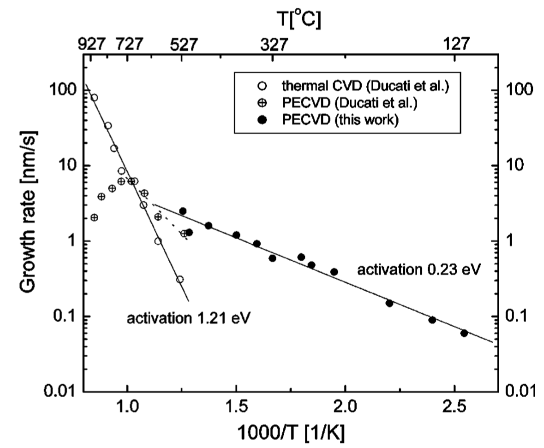
\includegraphics[width=8cm]{src/fig/fig38.png}
\caption{The activation energy in thermal-CVD and PE-CVD\textsuperscript{[22]}}
\end{figure}
With the assist of Hofmann’s low-temperature experiment result, we can get the essential rate constant values by fitting. 
\begin{figure}[H]
\centering
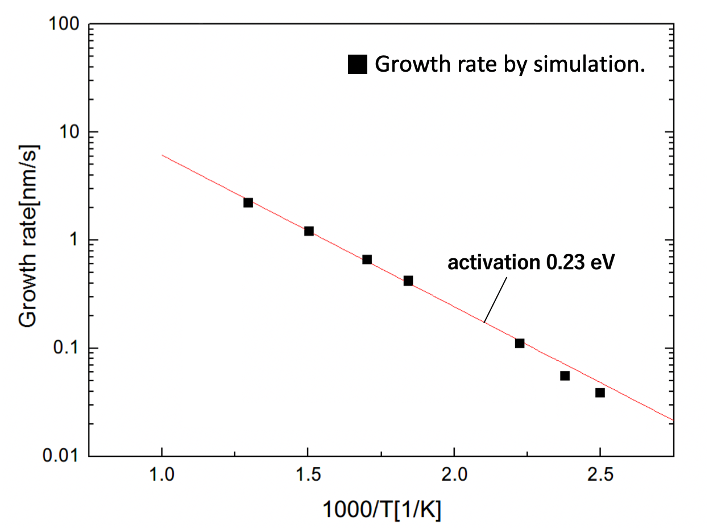
\includegraphics[width=8cm]{src/fig/fig39.png}
\caption{The fitted growth rate}
\end{figure}
Comparing the growth rates in fig. 3.9 (experimental result) and fig.3.10 (fitting result) the credibility of this CNT modeling is confirmed. It should be mentioned that in low-temperature region,  simulated length will be shorter than experiment result for the cone structure of CNF at lower temperature. Such deviation is because this calculation model assume  the tube shape, so $z$ ,the carbon atoms per meter in CNT will be larger than that in cone shape. 

\subsection{Ni silicidation\textsuperscript{[42]}}
There are tremendous investigation  into Ni silicidation in the field of electronic device. As we know, at a given high temperature, Ni silicidation occurs. Although Silicon atom is highly mobile, it is widely reported that that it is Ni atoms that being the dominant diffusing species in the phases in the Ni–Si system\textsuperscript{[43]}. According to Ni–Si binary phase, interphases including $\mathrm{Ni_{2}Si}$, $\mathrm{NiSi}$, $\mathrm{NiSi_{2}}$, $\mathrm{Ni_{5}Si_{2}}$ , $\mathrm{Ni_{3}Si}$ exist. However, the sequence of phases formed during silicidation does not necessarily follow the respective equilibrium diagrams, that is to say, some intermediate phases might be missing. Besides, in a low temperature range (200$\sim$325\(^\circ\)C), only $\mathrm{NiSi_{2}}$ exist on Si wafer, indicating that $\mathrm{NiSi_{2}}$ is the initial phase if at a higher temperature where Ni can proceed deeper in Silicon. With temperature increasing (300$\sim$400\(^\circ\)C), $\mathrm{NiSi}$  starts to form, followed by $\mathrm{NiSi_{2}}$ . The reaction kinetics of formation of the new phase can be categorized in to two (i) diffusion, (ii) nucleation. The formation of $\mathrm{Ni_{2}Si}$ and $\mathrm{NiSi}$ are diffusion-controlled while $\mathrm{NiSi_{2}}$  is nucleation controlled. 
Here we treat the Ni-silicidation issue based on the Fick’s law.

First, several assumptions are made to simplify the calculation. 
\begin{enumerate}[(i)]
\item Ni diffuses into Si.
\item One dimension diffusion.
\item Semi-infinite diffusion.
\item Only $\mathrm{Ni_{2}Si}$  phase is formed at T<300\(^\circ\)C
\end{enumerate}
\begin{figure}[H]
\centering
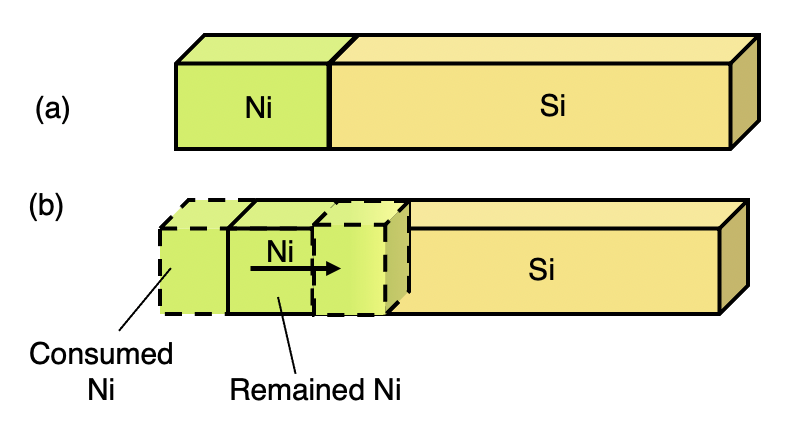
\includegraphics[width=8cm]{src/fig/fig40.png}
\caption{The one-dimension silicidation model at (a)initial, (b)in the process of annealing.}
\end{figure}
The diffusion coefficient $D$ of Ni is defined as,
\begin{equation}
D=D_{0} \exp \left(-E_{a} / k_{B} T\right)
\tag{3.2.18}
\end{equation}
Using the reported value $D= 2 \times 10^{-16} cm^{2}/sec$ at 200$^{\circ}$C and $E_{a}=1.5 eV$\textsuperscript{[42]}. Assume $D_{0}$ is constant at T<300$^{\circ}$C, thus the value of $D$ at 100$^{\circ}$C and 300$^{\circ}$C can be derived.
%对齐
$$\frac{\partial C}{\partial t}&=D\frac{\partial ^{2}C}{\partial x^{2}}$$
\begin{equation}
\begin{array}{lc}
\mathrm{Initial\quad condition}&:\qquad\qquad C(x,0)=0 \\
\mathrm{Boundary\quad condition\quad I}&:\qquad\qquad C(0,t)=C_{0}\\
\mathrm{Boundary\quad condition\quad I\hspace{-1pt}I}&: \qquad\qquad C(d_{Si},t)=0
\end{array}
\tag{3.2.19}
\end{equation}
General solution:
\begin{equation}
C(x, t)=C_{0} \operatorname{erfc}(x/2 \sqrt{D t})
\tag{3.2.20}
\end{equation}
Thus the concentration profile of Ni in Si is obtained. The integration of $C(x,t)$ from $0$ to $d_{Si}$ at certain moment(e.x. $t=1$ min) is the total consumption of Ni at that moment. By applying increasing $t$ into this integration eqaution the Ni consumption variation is obtained. The exact number of Ni atoms diffused into Si is not our interest but the relative ratio of remained Ni to initial Ni. If at the end of annealing there is still some pure Ni on the surface of Si particle, it's can be seen that the Ni is active as a catalyst. In the case of Ni:Si-NP, the size of Si is 20nm. The annealing time in PE-CVD is 15 minutes. 
\newpage
\subsection{Simulation result }
\begin{figure}[H]
\centering
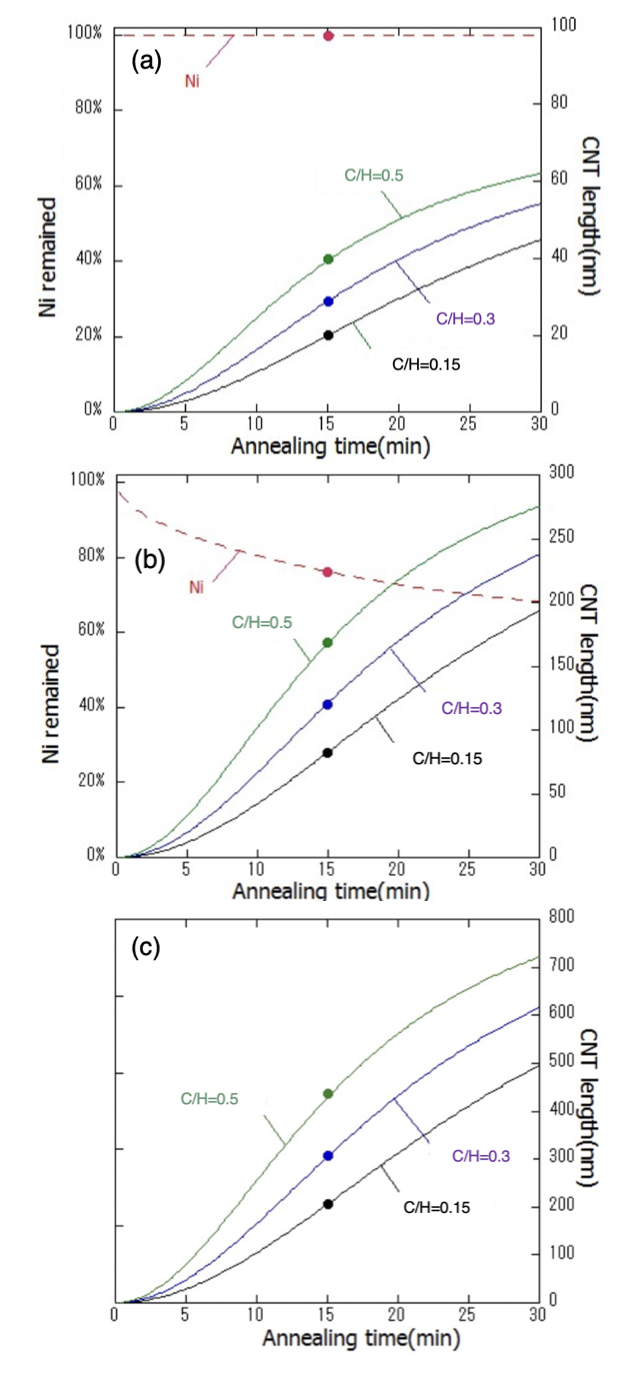
\includegraphics[width=8cm]{src/fig/fig41.png}
\caption{Competitive process between CNT growth and Ni silicidation at different annealing temperature of (a)100\(^\circ\)C (b)200\(^\circ\)C (c)300\(^\circ\)C}
\end{figure}

Except for temperature, another parameter that is controlled in this experiment is gas ratio. Due to the complexity of treating plasma, we assume that only temperature influence Ni silicidation. As to CNT calculation, It should be noted that gas ratio do influence the CNT growth for that the partial pressure of $\mathrm{C_{2}H_{2}}$ is changed. In addition, The gas ratio influence CNT growth in a way of changing  the  H species which is provide by $\mathrm{NH_{3}}$, however, not taken into this calculation due to the difficulty to quantify. The function of $\mathrm{NH_{3}}$ is to etch the competing amorphous carbon and graphitic phases. It may also have a role in keeping the gas side of the catalyst particle free of carbon, to allow continuing access of gas to the catalyst, and prevent it from becoming deactivated. While the flowrate of $\mathrm{NH_{3}}$ is changed to control the gas ratio, the plasma properties remains basically the same due to constant pressure.
\begin{table}[H]
\centering
\caption{Denotation of gas ratio}
\begin{tabular}{cc}
\toprule
Flow rate(sccm) & Denotation \\ \midrule
$\mathrm{C_{2}H_{2}}:\mathrm{NH_{3}=14:70}$ & C/H=0.15     \\
$\mathrm{C_{2}H_{2}}:\mathrm{NH_{3}=14:35}$ & C/H=0.3     \\
$\mathrm{C_{2}H_{2}}:\mathrm{NH_{3}=14:14}$ & C/H=0.5     \\ \bottomrule
\end{tabular}
\end{table}
Assuming CNT growth and Ni silicidation are independent from each other. On a Si nanoparticle($d_{Si}=20 nm$) with a grafted Ni cap($r_{Ni}=5 nm$)  we have the simulation result as fig.3.12 shows. At 100\(^\circ\)C, Ni silicidation is not occurring but due to the low temperature and the growth rate of CNT is suppressed as well. At 200\(^\circ\)C Ni silicidation occurs and CNT grows relatively faster. After annealing, the 300nm-long-CNT is grown and around 20\% of Ni cap is consumed. Unfortunately, when calculating the 300℃ case, Ni diffuse too fast that no longer meet the assumption of semi-finite diffusion.  




